گرامر سوال:
\begin{align*}
	S&\rightarrow Gx \\
	S&\rightarrow yGz \\
	S&\rightarrow Hz \\
	S&\rightarrow yHx \\
	G&\rightarrow w \\
	H&\rightarrow w \\
\end{align*}

ترنزیشن دیاگرم مربوط به گرامر فوق:

\qquad\qquad\qquad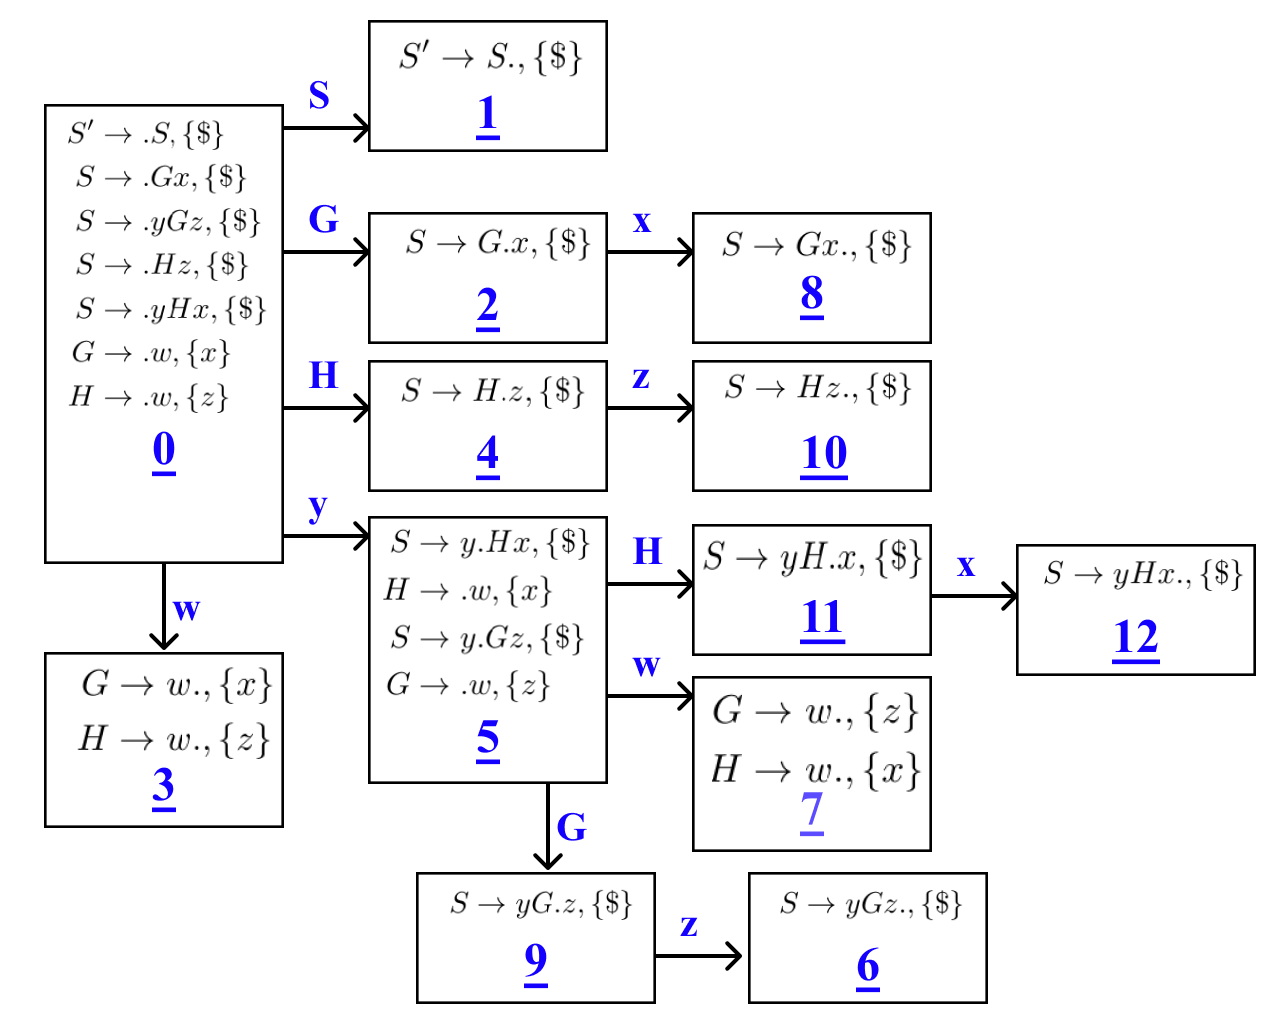
\includegraphics[width=0.7\linewidth]{figs/8.png}

\subsection*{الف}

جدول 
$LR(1)$
مربوط به گرامر فوق:

\qquad\qquad\qquad\qquad\qquad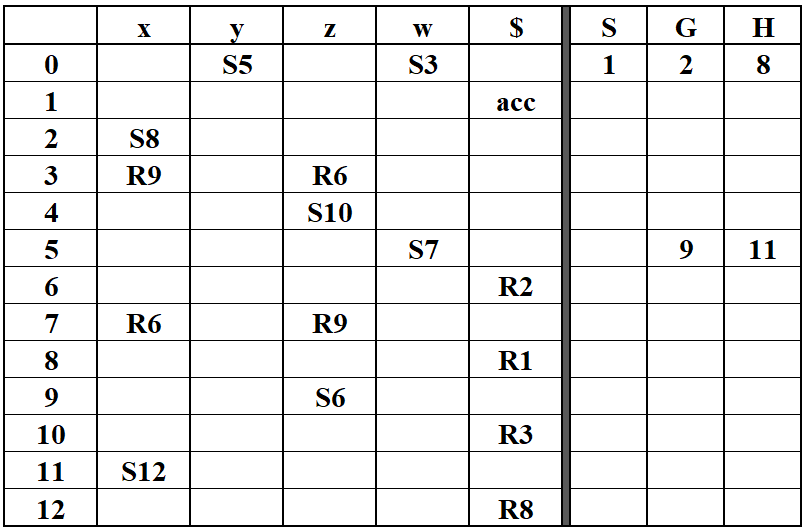
\includegraphics[width=0.5\linewidth]{figs/6.png}
\pagebreak

\subsection*{ب}

جدول 
$LALR(1)$
مربوط به گرامر فوق:

\qquad\qquad\qquad\qquad\qquad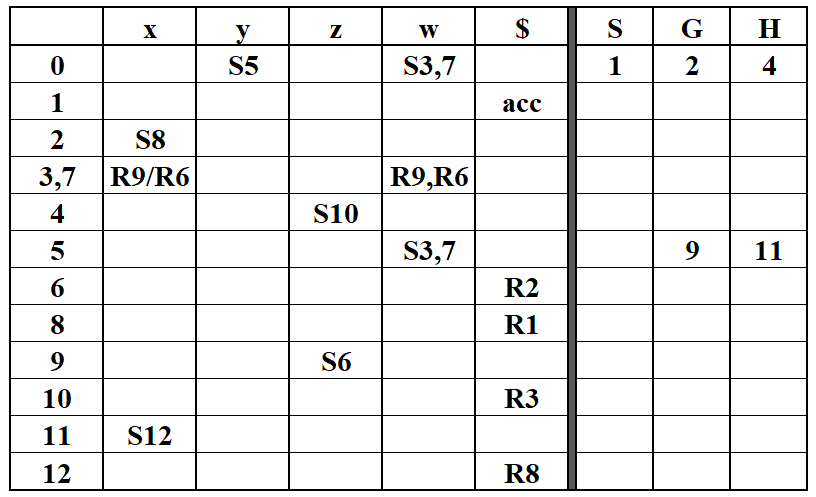
\includegraphics[width=0.5\linewidth]{figs/7.png}

\subsection*{ج}

همانطور که مشخص است، چون جدول 
$LR(1)$
تداخلی ندارد ولی جدول 
$LALR(1)$
دارای تداخل است. پس گرامر فوق از نوع 
$LR(1)$
است.



به عنوان مثال رشته ورودی 
$ywx\$$
را با استفاده از جدول فوق اگر پارس کنیم، داخل خانه 
$(37,x)$
به تداخل می‌خوریم.















